\documentclass{article}%
\usepackage[T1]{fontenc}%
\usepackage[utf8]{inputenc}%
\usepackage{lmodern}%
\usepackage{textcomp}%
\usepackage{lastpage}%
\usepackage{graphicx}%
%
\title{Statistics of chess games played by Stockfish}%
\author{Emilia Salvesen Kozarevic and Victor Windsor Torbjørn Norris}%
\date{\today}%
\maketitle%
%
\begin{document}%
\normalsize%
\section{Section one {-} Figures:}%
\label{sec:Sectionone{-}Figures}%
The following are figures:%
\subsection{Statistics over games won, tied and lost}%
\label{subsec:Statisticsovergameswon,tiedandlost}%


\begin{figure}[h!]%
\ \hspace*{-5cm}%
\centering%
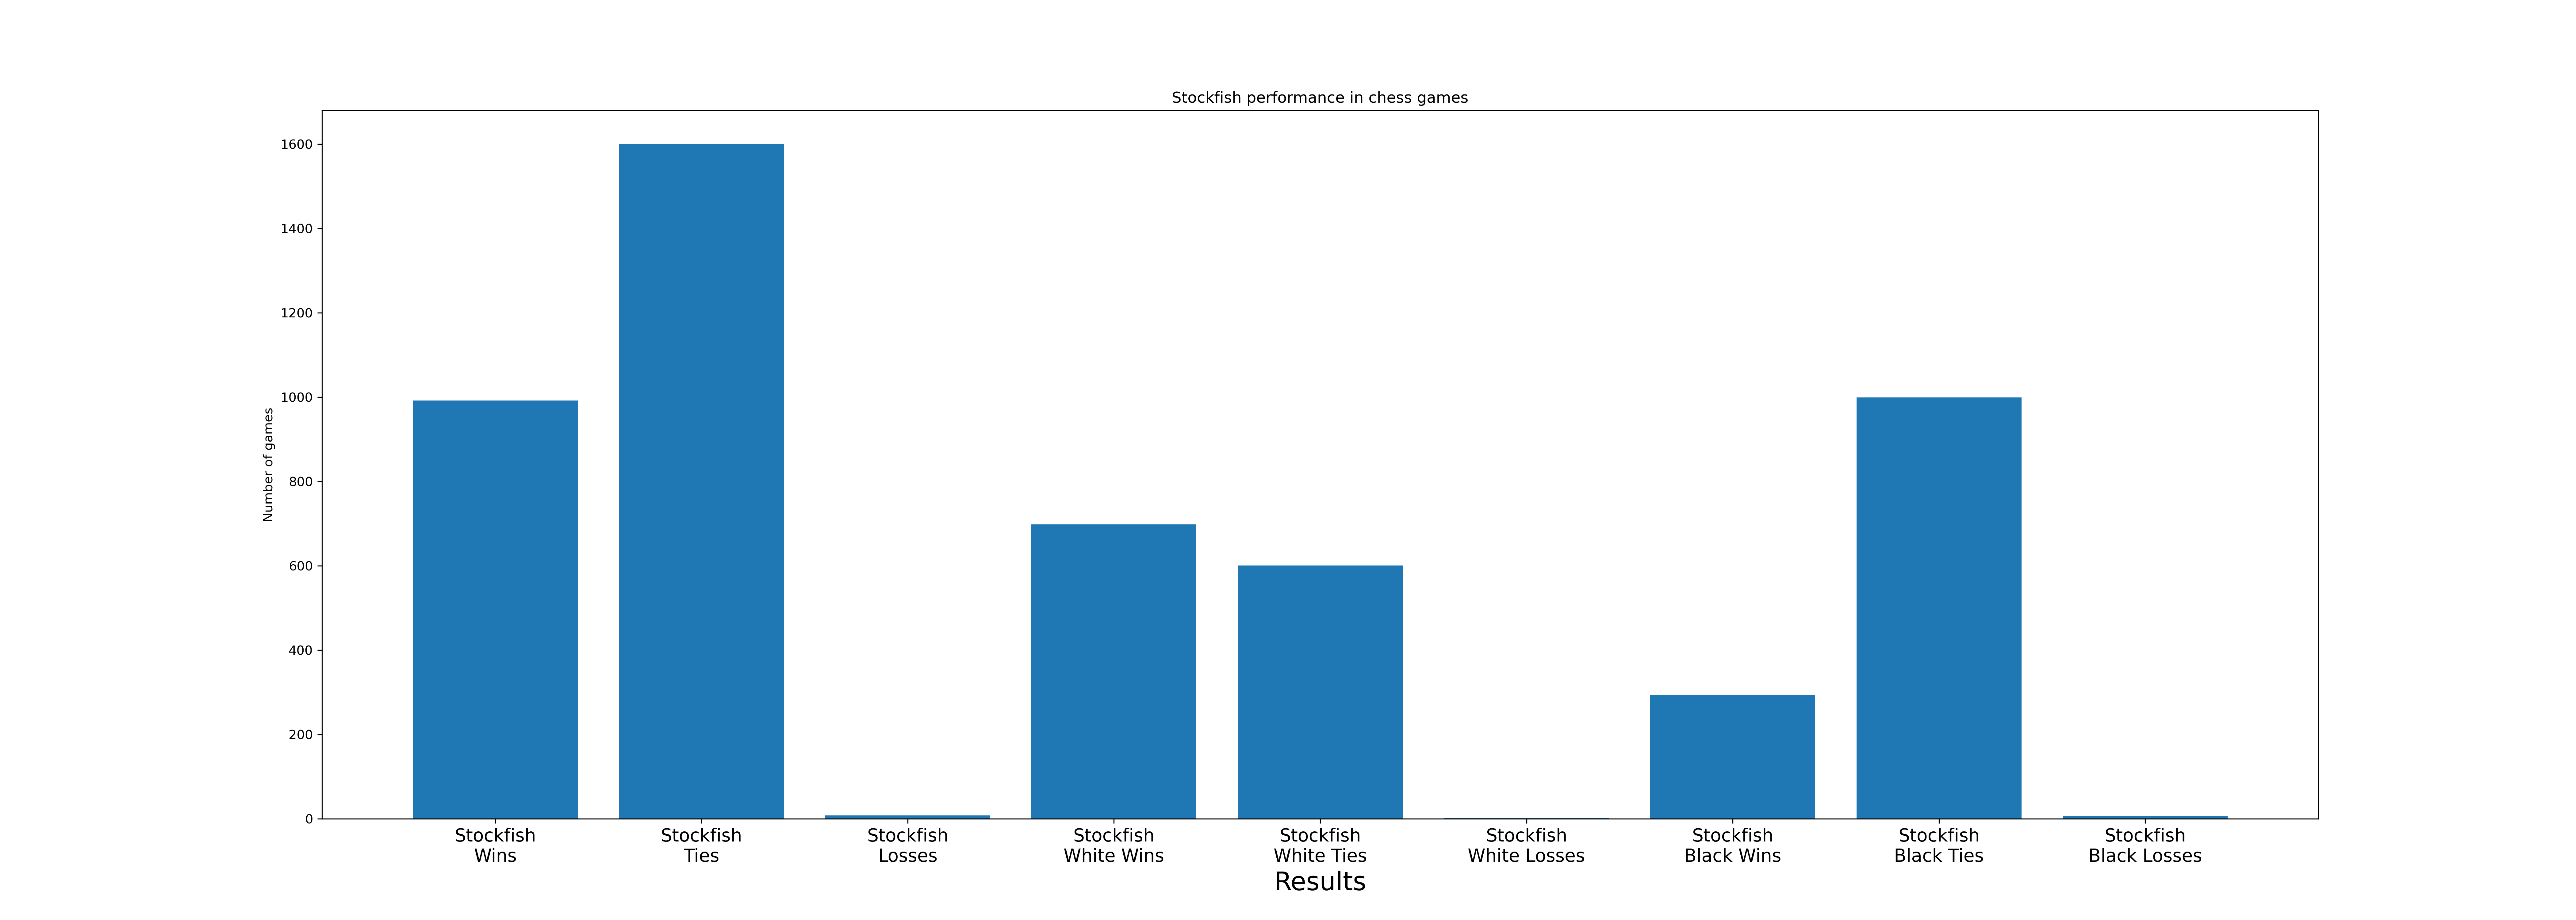
\includegraphics[width=1.8\textwidth]{stockFish.png}%
\caption{A plot of Stockfish performance in chess games. In total, with white and with black pieces.}%
\end{figure}

%
\subsection{Lineplot}%
\label{subsec:Lineplot}%


\begin{figure}[h!]%
\ \hspace*{-4cm}%
\centering%
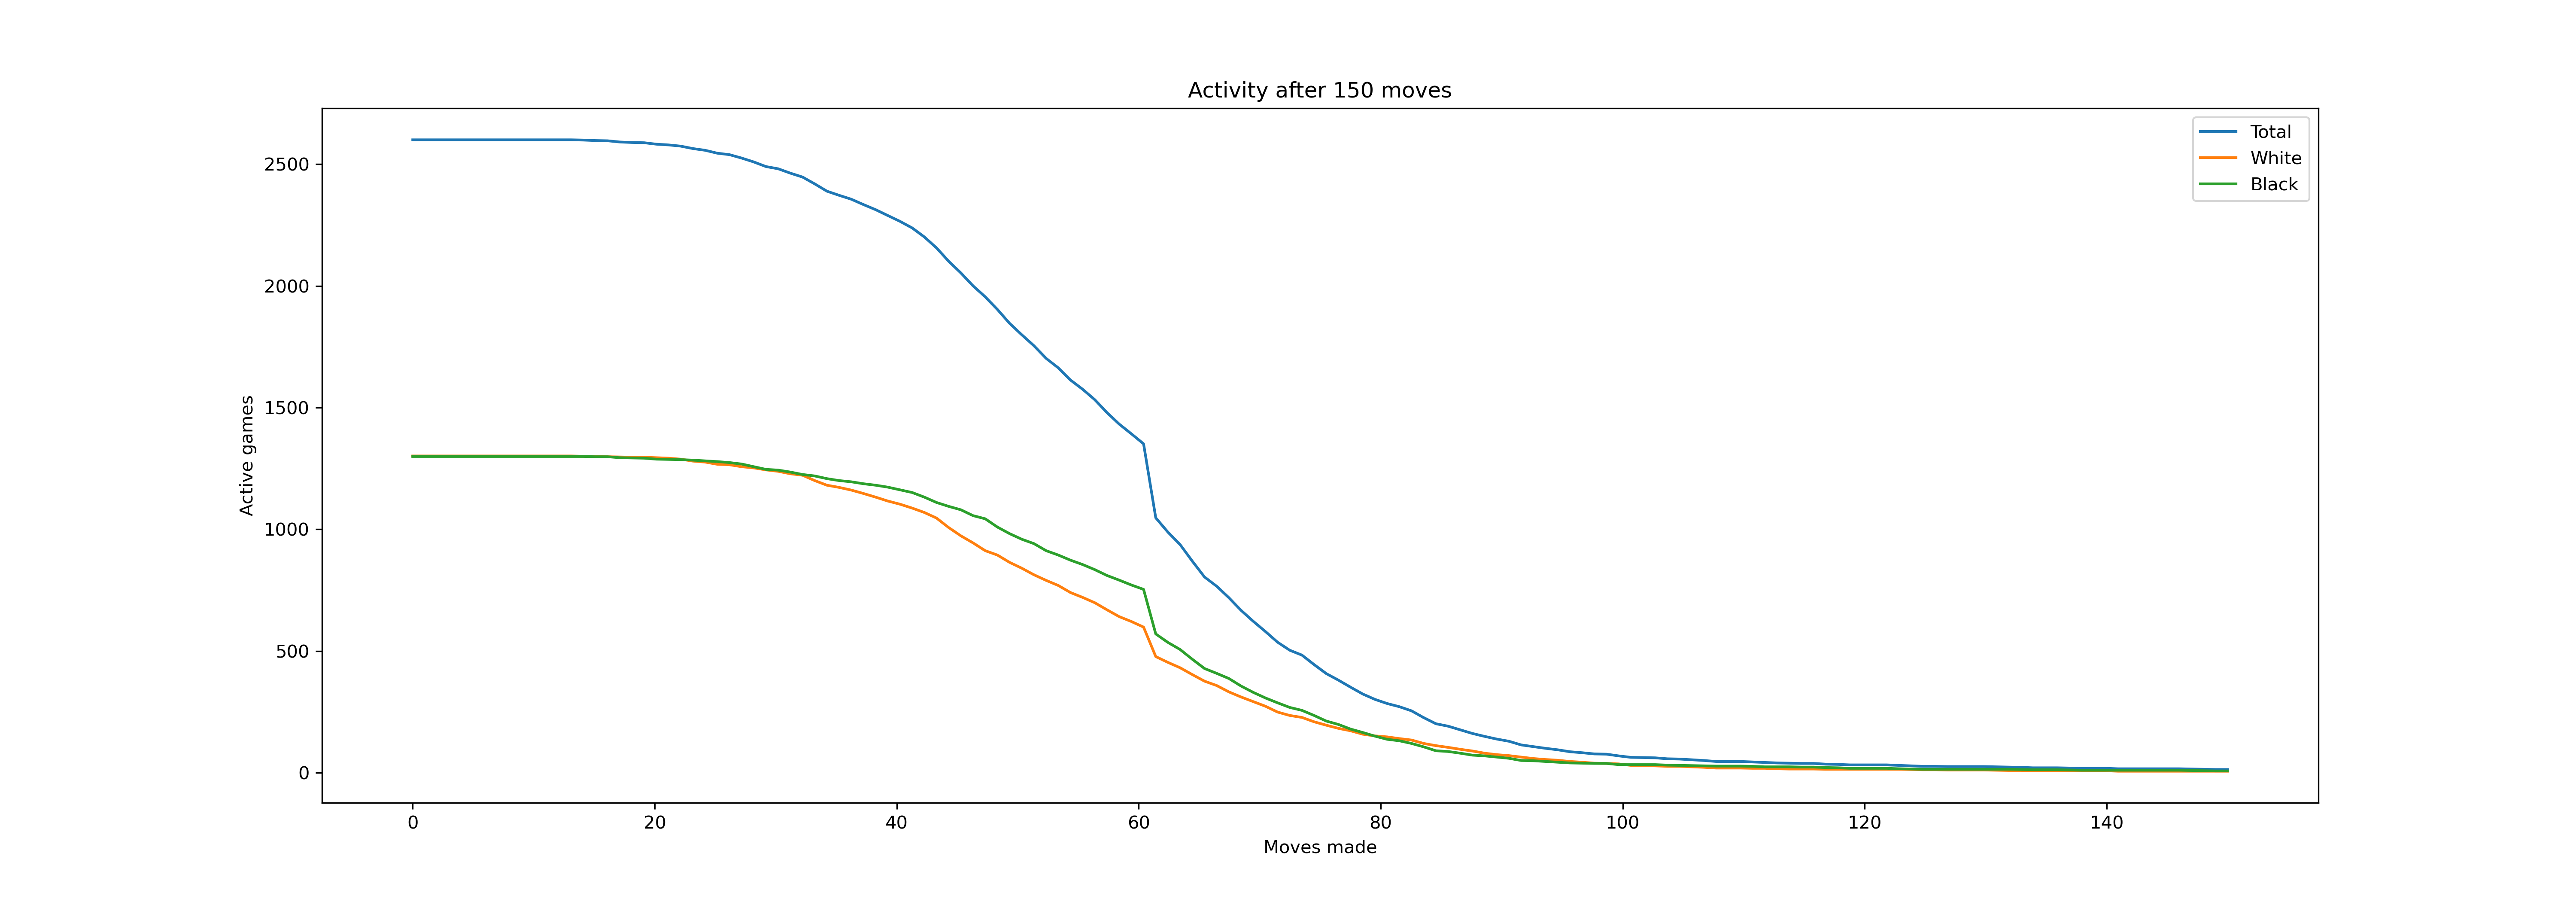
\includegraphics[width=1.8\textwidth]{ActiveGamesLine.png}%
\caption{A plot of active games after x moves. Shows the plot for total games, games played as white by stockfish and as black by stockfish}%
\end{figure}

%
\subsection{Statistics of mean and standard deviation:}%
\label{subsec:Statisticsofmeanandstandarddeviation}%


\begin{figure}[h!]%
\ \hspace*{-3cm}%
\centering%
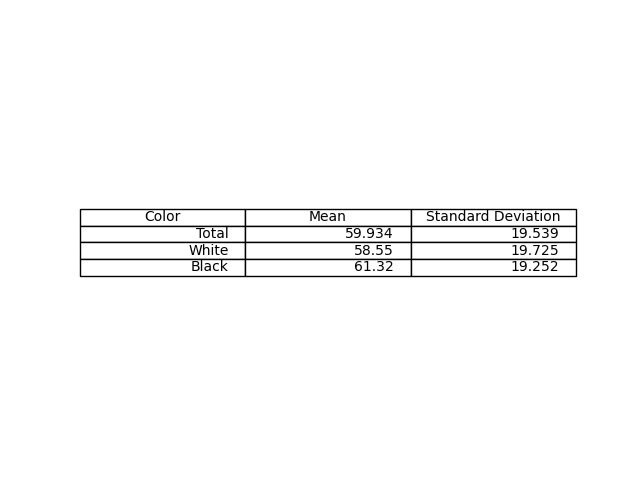
\includegraphics[width=1.4\textwidth]{table.png}%
\caption{Stats for all games, white games and black games by stockfish}%
\end{figure}

%
\subsection{Statistics over most popular openings}%
\label{subsec:Statisticsovermostpopularopenings}%


\begin{figure}[h!]%
\ \hspace*{-5cm}%
\centering%
\includegraphics[width=1.8\textwidth]{NormalOpenings.png}%
\caption{A table with the most popular openings, as well as stats for these}%
\end{figure}

%
\section{Section two {-} Opening Tree:}%
\label{sec:Sectiontwo{-}OpeningTree}%
The following section is a tree for a selected chess opening.%
\subsection{Opening tree}%
\label{subsec:Openingtree}%


\begin{figure}[h!]%
\ \hspace*{-2cm}%
\centering%
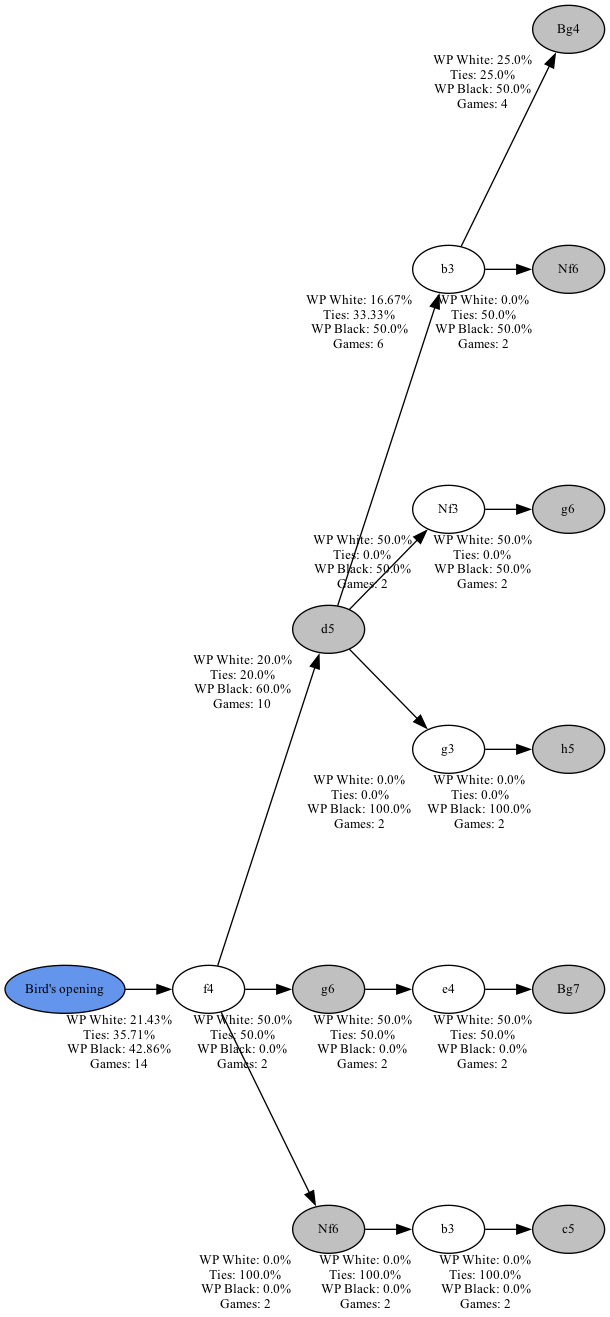
\includegraphics[width=0.7\textwidth]{OpeningTree.png}%
\caption{A plot of an opening tree}%
\end{figure}

%
\end{document}